% Created 2022-03-05 Sat 14:51
% Intended LaTeX compiler: pdflatex
\documentclass[11pt,a4paper]{article}
\usepackage[utf8]{inputenc}
\usepackage[T1]{fontenc}
\usepackage{fixltx2e}
\usepackage{graphicx}
\usepackage{longtable}
\usepackage{float}
\usepackage{wrapfig}
\usepackage{rotating}
\usepackage[normalem]{ulem}
\usepackage{amsmath}
\usepackage{textcomp}
\usepackage{marvosym}
\usepackage{wasysym}
\usepackage{amssymb}
\usepackage{hyperref}
\usepackage{mathpazo}
\usepackage{color}
\usepackage{enumerate}
\usepackage{lastpage}
\definecolor{bg}{rgb}{0.95,0.95,0.95}
\tolerance=1000
            \setlength{\parindent}{0pt}
\usepackage[danish]{babel}
\usepackage{pdfpages}

\linespread{1.1}
\hypersetup{pdfborder=0 0 0}

\setlength{\parindent}{0pt}
\usepackage{fancyhdr}
\usepackage{lipsum}
\fancyfoot{}
\pagestyle{fancy}
\rfoot{Page \thepage \hspace{1pt} of \pageref{LastPage}}
\author{Aksel Mannstaedt}
\date{}
\title{Virkeligt Hurtige Fourier Transformationer}
\hypersetup{
 pdfauthor={Aksel Mannstaedt},
 pdftitle={Virkeligt Hurtige Fourier Transformationer},
 pdfkeywords={},
 pdfsubject={},
 pdfcreator={Emacs 29.0.50 (Org mode 9.6)}, 
 pdflang={Danish}}
\begin{document}

\maketitle
\noindent\rule{\textwidth}{0.5pt}
\begin{center}
Kode med tekst og grafer - \url{https://nbviewer.org/github/unic0rn9k/fourier-notebook/blob/master/README.ipynb}

github repo - \url{https://github.com/unic0nr9k/fourier-notebook}

\bigskip

Jeg vil stærkt opfordre til at prøve at downloade notebooken og prøve at eksperimentere med at kombinere forskellige andre bølger for at se at min FFT implementering virkeligt virker.
\end{center}

\noindent\rule{\textwidth}{0.5pt}

\setcounter{tocdepth}{2}
\tableofcontents

\newpage

\section{Teori}
\label{sec:org4af6088}
\subsection{Rekursion og funktionel programmering}
\label{sec:org0708a7b}

Rekursion er helt simpelt, en funktion der kalder sig selv.
Dette bliver brugt meget i funktionel programmering.

Funktionel programmeringssprog er et paradigme kendetegnet ved
et fokus på funktioner i stedet for objekter og kontrol strukturer. \footnote{\url{https://en.wikipedia.org/wiki/Functional\_programming}}

\bigskip

Fordele ved funktionelle programmeringssprog er at de er designet til at formindske side effects,
og derved uforudventet adfærd.
Side effects er defineret som en operation der muterer data udenfor den funktion der ejer data'en.
Dette vil altså siges, at hvis man har en funktion der tager en pointer til en værdi og så ændrer på
den værdi via pointeren, vil det være en side effekt af funktionen.

Dette kan skabe uforudventet adfærd i et program og vil derfor typisk gerne undgås.

Fuldkommen funktionelle programmeringssprog er sprog, hvor man ikke kan mutere data overhovedet.
Det betyder altså, at hvis man for eksempel vil lave et for loop, er man nødt til at bruge rekursion.

Fuldkommen funktionelle programmeringssprog bliver ikke rigtigt anvendt i praksis,
men de er dog stadig relevante at skrive om, da de er tættere på matematisk notering
end traditionelle programmeringssprog.

I min case har jeg anvendt fuldkommen funktionel psudo kode til at lave en model
for hvordan jeg ville strukturere min implementering af Cooley-Tukey FFT algoritme.

\subsection{Hvad er en Fourier transformation?}
\label{sec:orgae084c4}
\newpage

En Fourier transformation er en vektor transformation (der i øvrigt også kan udvides til n-dimensionelle tensore)
der blandt andet kan anvendes til at transformere et polynomium,
repræsenteret som en koefficient-vektor, til en punkt-vektor repræsentation.
Dette er også ækvivalent til en time to frequency -domain transformation.
Altså den også kan anvendes som en transformation af bølger repræsenteret som intensitet over tid til intensitet over frekvens.
Her vil jeg lige pointere at alle disse operationer er ækvivalente, altså det er bare forskellige måder at repræsentere, tænke på og visualizere den samme transformation.
Jeg vil primært fokusere på bølge repræsentationen af Fourier transformationen, der jeg synes den er lidt nemmere at forstå.

Her er som eksempel en bølge og dens tilhørende Fourier transformation.
Bølgen er en kombination af en 7, 14 og 19 frekvens bølge (Frekvensen er enhedsløs der den er bølge længde over vektorens længde).

\begin{center}
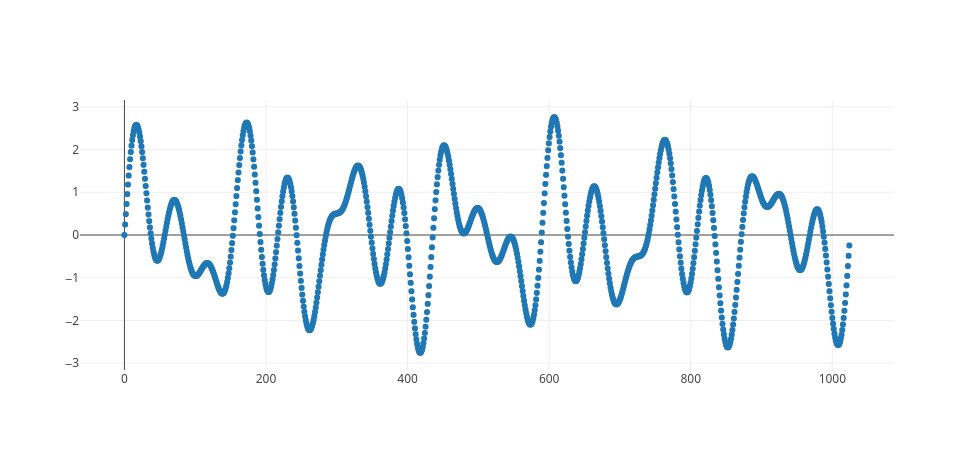
\includegraphics[width=.9\linewidth]{./source_plot2.png}
\end{center}

Her kan man altså se der ligger lokale maksimal punkter lige omkring 7, 14 og 19 på x-aksen.
\begin{center}
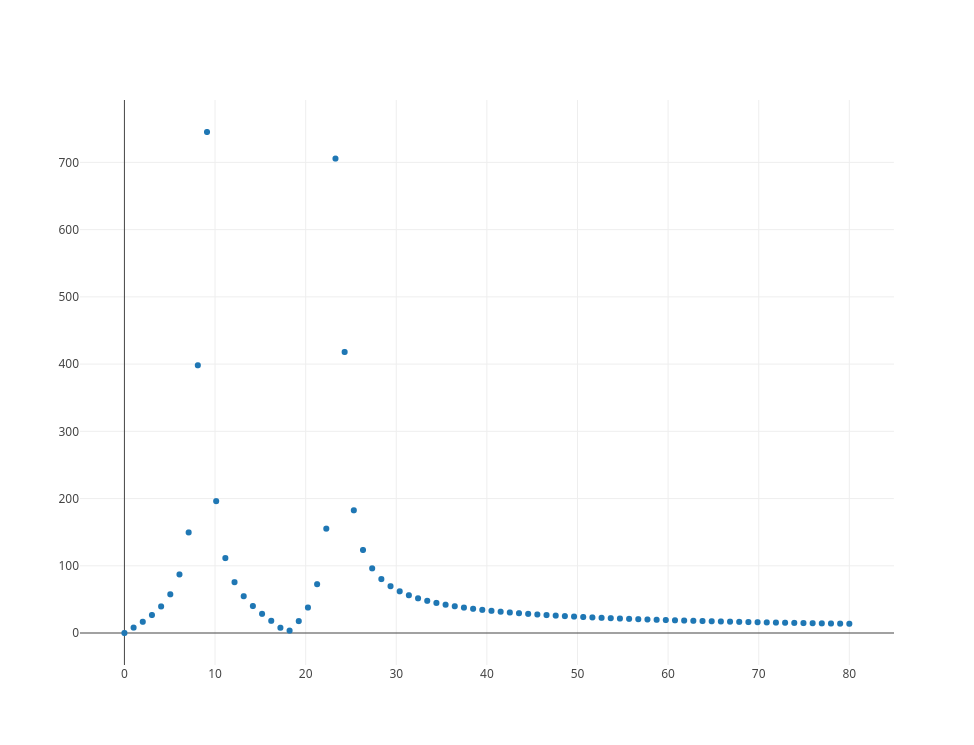
\includegraphics[width=.9\linewidth]{./plot2.png}
\end{center}

\bigskip

\subsection{DFT}
\label{sec:org8bcd833}
DFT er kort for diskret Fourier transformation, og var den originale formel opdaget af Joseph Fourier i 1830.
Han fandt ud af, hvordan man kunne lave de her transformationer, før man kunne udregne dem på computere,
eller havde nogen praktisk anvendelse til dem\footnote{\url{https://en.wikipedia.org/wiki/Joseph\_Fourier}}.

Her er f frekvens, t er tid, g er en sammensat bølge funktion og \(\hat{g}\) er den Fourier transformerede funktion af g.
$$
\hat{g}(f) = \int_{+\infin}^{-\infin{}} g(t) \cdot e ^{-2\pi ift}dt
$$

Formlen ovenfor viser hvordan en diskret Fourier transformation kan udregnes,
den kan se lidt skræmmende ud, men er nem nok at forstå når man lige har styr på et par koncepter indenfor matematik.

\bigskip

\subsubsection{Komplekse tal og Euler's identitet}
\label{sec:org077a1ac}

Et komplekst tal er et tal bestående af en imaginær del og en reel del (summen af dem).
Den imaginære del af det komplekse tal er defineret som produktet af et
virkeligt tal og \(i\).

\(i\) er defineret som kvadratroden af -1. (altså det findes ikke).

Det giver måske ikke lige umiddelbart så meget mening, men en nem måde at tænke på det,
er som en 2d vektor der har nogen specielle regne regler.

For eksempel vil \((0 + 1i)^2\) være -1, da \(i^2\) skal give -1.

Komplekse tal bliver typisk også visualiseret som en 2d-vektor,
hvor den reelle del er på x-aksen, og den imaginære del er på y-aksen.

Her vil det svares til en \(90^\circ\) rotation, i det komplekse plan, at gange med \(i\).

$$
(1 + 0i) \cdot i = 0 + 1i
$$
$$
(0 + 1i) \cdot i = -1 + 0i
$$
$$
(-1 + 0i) \cdot i = 0 - 1i
$$
osv\ldots{}

\newpage

For at kunne forstå Fourier transformeringer er det vigtigt at forstå Euler's identitet,
som er defineret som

$$
e^{\pi i} = -1
$$

Dette udtryk kommer af at \(e^x\) er sit eget derivativ (\(e\) er Euler's konstant \footnote{\url{https://en.wikipedia.org/wiki/Euler\%27s\_constant}}),
det vil altså siges at \(\frac{d}{dx}e^{kx} = k\cdot e^{kx}\), hvor k er en konstant.

Altså man kan sige at \(e^{kx}\) bevæger sig i retningen \(k \cdot e^{kx}\).
Det betyder at hvis vi bytter \(k\) ud med \(i\), må \(e^{ix}\) bevæge sig mod en \(90^\circ\) rotation med en hastighed af en radian per x.

Her vil en halv rotation derfor svare til \(x=\pi\) og vi kan derved konkludere at \(e^{\pi i} = -1\).

\subsubsection{Uddybning af Fourier transformation}
\label{sec:orgd2b373b}

Den inderste del af den diskrete Fourier transformering kan ses lidt som et prik produkt
$$
f(t) = g(t) \cdot e ^{-2\pi ift}
$$

Her vil det virkelige komponent af \(f(t)\) være større når intensiteten af \(g(t)\)
matcher den der ville findes hvis frekvensen af \(g\) var \(f\).

Dette kan intuitivt forstås, som at når \(t\) værdier ligger i bølgedale, vil \(e^{-2\pi ift}\) være negativ
og derfor vil \(f(t)\) være positiv hvis \(g(t)\) også er negativ.

\(-2\pi\) sikre at en forøgelse af en tidsenhed svarende til en periode med frekvensen \(f\) også vil resultere
i en fuld rotation af \(e^{-2\pi ift}\).

Det skal være et integrale for at sikre at frekvensen matcher over en længere periode.
Altså hvis man ikke brugte integralet,
ville enkelte punkter der matcher dem fra frekvensen \(f\) også resultere i en høj værdi på \(\hat{g}(f)\).

\bigskip

DFT algoritmen har en algoritmisk kompleksitet på \(O(n^2)\) der \(\hat{g}\) er en funktion af både tid og frekvens.

\newpage

\subsection{FFT}
\label{sec:org8b6a31b}

\subsubsection{Koefficient to punkt repræsentation}
\label{sec:org6edc24d}

Fourier transformeringen svares ikke kun til en tids til frekvens domæne transformering,
men også til en koefficient til punkt repræsentation,

givet en bølge repræsenteret som en vektor af intensitet over tid
$$
\vec{b} = [0, 1, 2, 3]
$$

vil kunne repræsenteres som et polynomium
$$
b(x) = x + 2\cdot x^2 + 3\cdot x^3
$$

her vil det gælde at
$$
\hat{b}(x) = b((-i)^x)
$$

\textbf{DFT eksempel med Julia:}
\begin{verbatim}
julia> b(x) = 2*x^2 + 3*x^3 + x
b (generic function with 1 method)

julia> for n in 0:3
            println(b((-im)^n))
       end
 6 + 0im
-2 + 2im
-2 + 0im
-2 - 2im

julia> fft([0, 1, 2, 3])
4-element Vector{ComplexF64}:
  6.0 + 0.0im
 -2.0 + 2.0im
 -2.0 + 0.0im
 -2.0 - 2.0im
\end{verbatim}

I eksemplet over kan man tydeligt se \(O(n^2)\) kompleksiteten,
der funktionen \(b\), har \(n\) led der skal udregnes
og \(b\) sig selv skal også computeres \(n\) gange.

Polynomier af en lige grad er spejlet om y-aksen.
Polynomier af en ulige grad er spejlet om y-aksen og x-aksen.

\begin{verbatim}
plot(x^2) + plot(x^3, color='red') + plot(x^4) + plot(x^5, color='red') + plot(x^6) + plot(x^7, color='red')
\end{verbatim}

\begin{figure}[htbp]
\centering
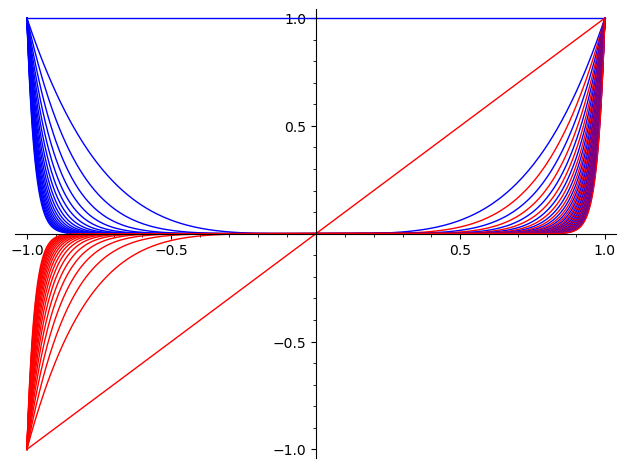
\includegraphics[width=.9\linewidth]{even_and_odd.png}
\caption{Lavet med sagemath}
\end{figure}

Vi kan udnytte den egenskab af polynomier ved at splitte vores polynomium op i ulige og lige led
og derved evaluer polynomiet på mindre punkter.

\textbf{Eksempel:}
$$
f(x) = (3x^2 + 4x^3 + 2x^4 + x^5) = (3x^2 + 2x^4) + x(4x^2 + x^4)
$$

$$
f_{lige}(x) = 3x + 2x^2
$$

$$
f_{ulige}(x) = 4x + x^2
$$

Bemærk at graden af alle ledn'e er divideret med 2 og en er trukket fra graden af det ulige polynomium.
Dette gør at vektor repræsentationen af \(f_{lige}\) og \(f_{ulige}\) vil svares til alle de lige/ulige værdier fra \(\vec{f}\),
samlet i nye vektorer. Her vil dimensionen af \({\vec{f_{lige}}}\) og \({\vec{f_{lige}}}\) altså være \(n/2\), hvor \(n\) er dimensionen af \(\vec{f}\).

$$
f(x) = f_{lige}(x^2) + x \cdot f_{ulige}(x^2)
$$

For negative x-værdier, er det altså kun \(f_{ulige}\) der skal sættes i minus,
der de lige er spejlet om y-aksen.

$$
f(-x) = f_{lige}(x^2) - x \cdot f_{ulige}(x^2)
$$

Her fra bliver \(f\) delt op i lige og ulige koefficienter rekursivt indtil den skal evalueres på et punkt.

For at kunne fortsætte herfra skal vi kunne generare \(n\) tal, der alle giver 1 når de bliver opløftet i \(n\)'de.
Her skal \(n\) altid være \(2^{noget}\), for at polynomiet kan deles op i positive og negative par rekursivt ned til en koefficient.

For at kunne skal vi finde et sæt af unikke \(x\) værdier der kan opløftes i \(2^n\) og stadig give et positivt og negativt par.
Her er der nogen specielle tal der hedder the n'th roots of unity, der opfylder disse krav.

\textbf{n'th root of unity:}

Her anvendes Euler's formel til at udregne \(n\) komplekse tal der er liggeligt fordelt på en enheds cirkel.

\begin{figure}[htbp]
\centering
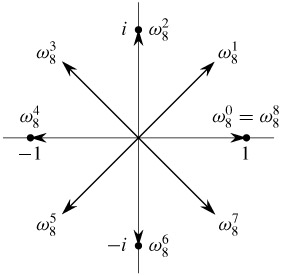
\includegraphics[width=.9\linewidth]{./nth_root_of_unity.jpg}
\caption{\url{http://www.euroinformatica.ro/documentation/programming/!!!Algorithms\_CORMEN!!!/images/fig853\_02.jpg}}
\end{figure}

$$
\omega_n = e^{\frac{-2\pi i}{n}}
$$

$$
-\omega_n^j = \omega_n^{j+\frac{n}{2}}
$$

I min kode har jeg divideret \(n\) med 2 i de rekursive kald i stedet for at tage \(\omega\) i anden, der det vil give det same resultat.
\begin{equation}
\begin{split}
\omega_n^2 &= e^{\frac{-2\pi i}{n}} \\
&= e^{\frac{-2\pi i \cdot 2}{n}} \\
&= e^{\frac{-2\pi i}{n/2}} \\
&= \omega_{\frac{n}{2}}
\end{split}
\end{equation}

\(\vec{f}\) vil blive udregnet ved at evaluere \(f\) for vær værdi af \(j\), hvor \(j\) antager værdierne fra 0 til \(n/2\).

$$
f(\omega^{j+\frac{n}{2}}_n) = f_{lige}(\omega^2) - \omega \cdot f_{ulige}(\omega^2)
$$
$$
f(\omega^j_n) = f_{lige}(\omega^2) + \omega \cdot f_{ulige}(\omega^2)
$$

Her bliver \(f(\omega_n^j)\) evalueret rekursivt indtil et 0 grads polynomium er tilbage, hvor FFT'en skal returnere koefficient af polynomiet.
De negative evalueringer bliver placeret på højrehåndssiden af den resulterende vektor og de positive på højre side.

\section{Tooling (programmering)}
\label{sec:org0e66b7a}
Jeg valgte at skrive koden til denne case i rust, da jeg er komfortabel med sproget,
og gerne ville eksperimentere med at lave en hurtig implementering af Cooley-Tukey algoritmen.

Rust er et rigtigt hurtigt sprog, dette skyldes blandt andet at det bruger llvm som backend,
men også rust's brug af zero-cost-abstractions.

Jeg valgte at skrive koden i en jupyter notebook, da jeg ikke havde nogen egentlig
applikation af min kode i tankerne under forløbet.
Det viste sig også at være super praktisk til at lave TDD (test driven development),
da det betød jeg kunne smide nogen grafer ind, og have dem opdateret i næsten realtime,
mens jeg arbejdede på implementeringen af FFT algoritmen.

\subsection{Rust sprog paradimer}
\label{sec:org71102bc}
Rust er et memory-safe programmeringssprog,
hvilket betyder at det by-default ikke lader en skrive koder, der kan resultere i undefined-behavior\footnote{\url{https://doc.rust-lang.org/reference/behavior-considered-undefined.html}}.
Dette betyder at rust har en borrow-checker der ikke lader ens kode compile' hvis det bryder nogen regler defineret i rust sprog specifikationerne.
Man kan for eksempel ikke bruge en reference i flere funktioner på en gang, og alle værdier skal makkeres med
en mutability specificer, der bestemmer om man kan ændre på den. Derudover introducere rust også et koncept der hedder lifetimes,
som kort sagt betyder at kompileren sikre at man ikke kan bruge references til værdier der er blevet deallokeret.

\bigskip

Disse regler er ikke absolutte. Man kan makkere kode som `unsafe` for at slippe uden om reglerne introduceret af compileren.

I min kode har jeg for eksempel valgt at lave en meget unsafe implementering af FFT algoritmen,
men har så lavet en safe wrapper til den, der sikre at man ikke kan introducere undefined behavior i sin kode ved brug af min algoritme.

\section{Inplace operationer og statisk allokering}
\label{sec:org5c1b24c}

\section{Twiddle factor}
\label{sec:org40765a8}

\section{Bibliografi}
\label{sec:orgb7a2c04}

1: Undefined-behavior - \url{https://doc.rust-lang.org/reference/behavior-considered-undefined.html}

2: Funktionel programmering - \url{https://en.wikipedia.org/wiki/Functional\_programming}

3: Fourier - \url{https://en.wikipedia.org/wiki/Joseph\_Fourier}

4: Euler's konstant - \url{https://en.wikipedia.org/wiki/Euler\%27s\_constant}


\section{Bilag}
\label{sec:org168d664}

Kode som pdf vedhæftet på næste side\ldots{}
Grafer kan ikke vises i pdf'en, derfor anbefaler jeg at kigge på notebook'en linket til i toppen af dokumentet.

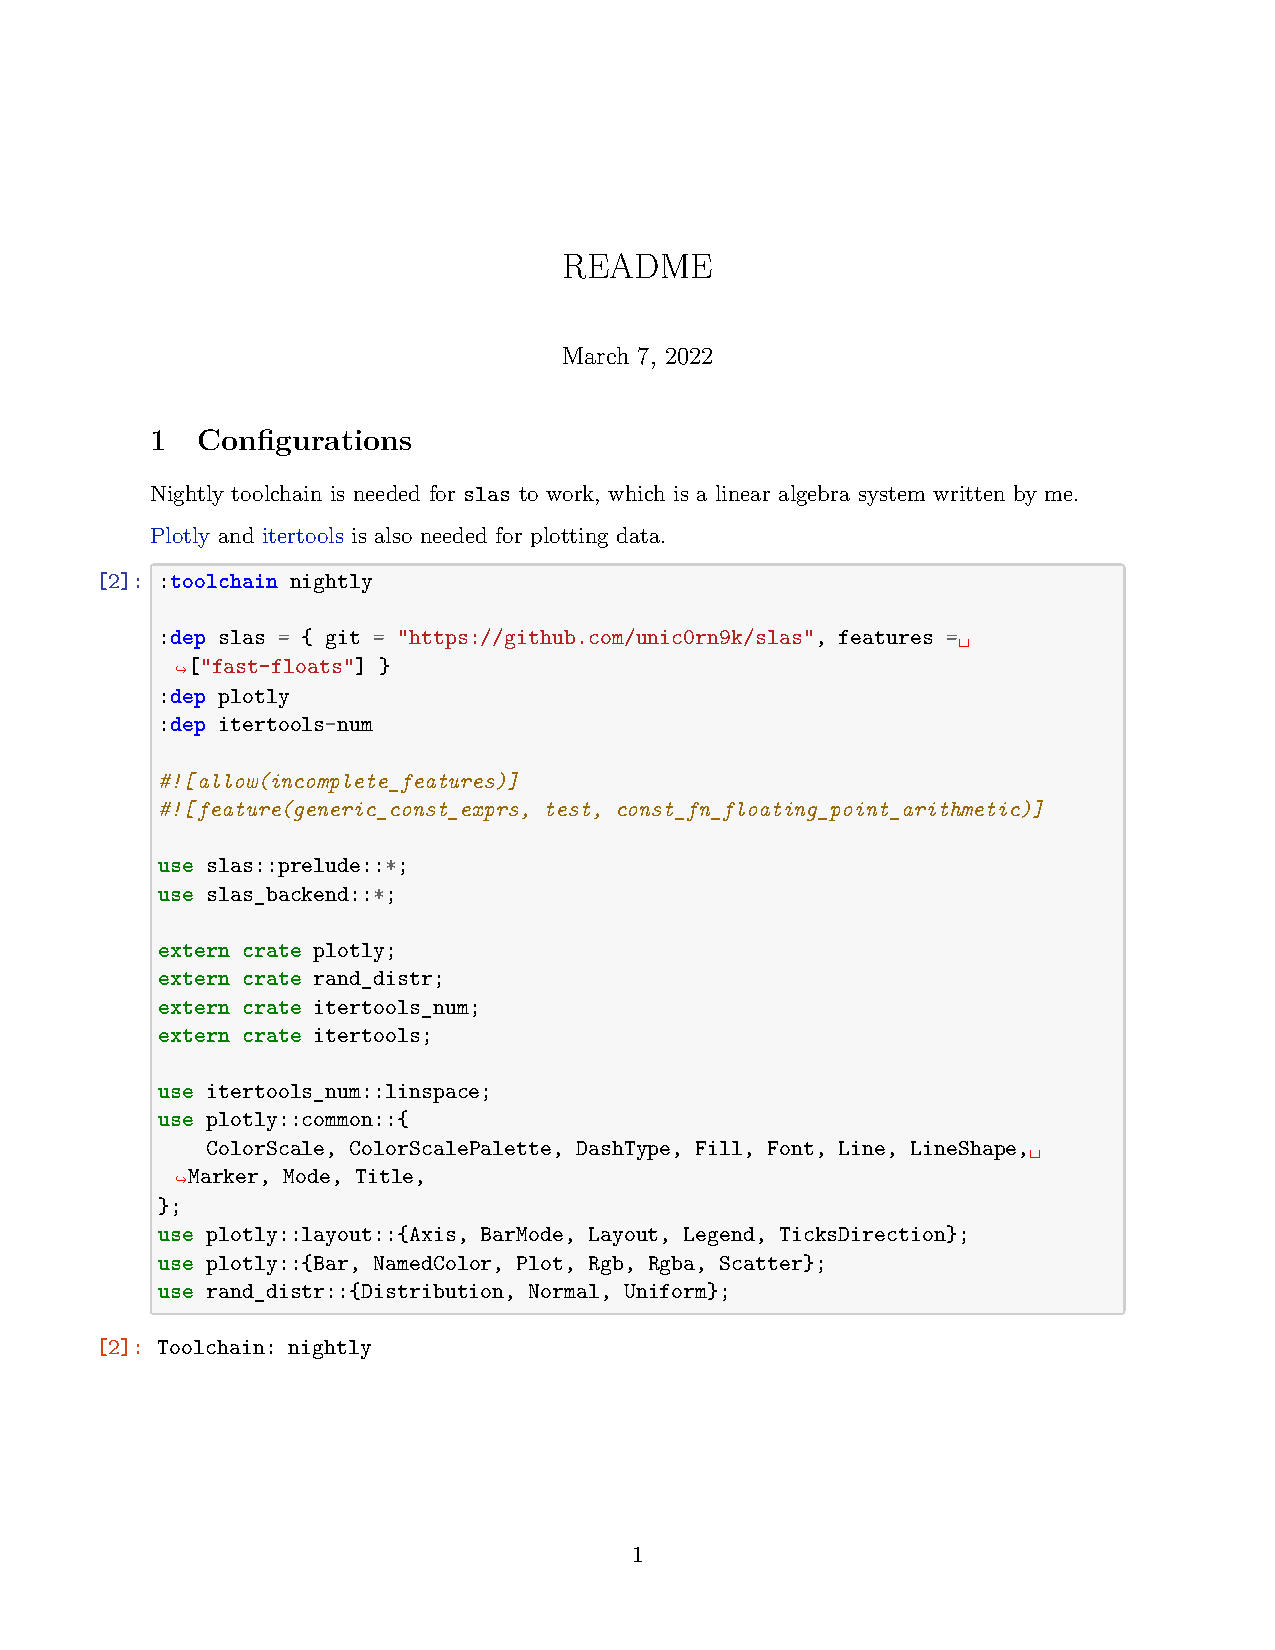
\includepdf[pages=-]{notebook.pdf}
\end{document}
